\documentclass[tikz]{standalone}
\usepackage{amsfonts}
\usepackage{amsmath}
\usepackage{amssymb}
\usepackage{tikz}

\begin{document}

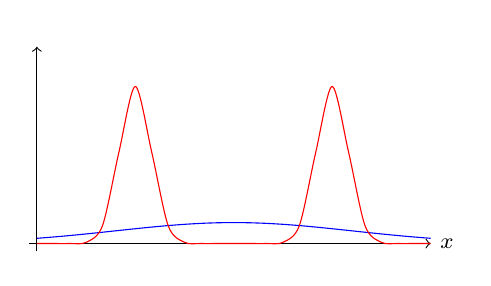
\begin{tikzpicture}
	%Axis
      \draw[->] (-0.1,0) -- (5,0) node[right] {\footnotesize{$x$}};
      \draw[->] (0,-0.1) -- (0,2.5) node[above] {};
      
      %Plots
      \draw[scale=1, domain=0:5,smooth,variable=\x,blue] plot ({\x},{  1/sqrt(2*pi*(1.5^2))*exp( -0.5*( (\x -2.5)^2 )/ (1.5^2) )   });
      \draw[scale=1, domain=0:5,smooth,variable=\x,red] plot ({\x},{  1/sqrt(2*pi*(0.2^2))*exp( -0.5*( (\x -1.25)^2 )/ (0.2^2) ) + 1/sqrt(2*pi*(0.2^2))*exp( -0.5*( (\x -3.75)^2 )/ 	(0.2^2) )   });
      
\end{tikzpicture}

\end{document}